\begin{figure}
\centering
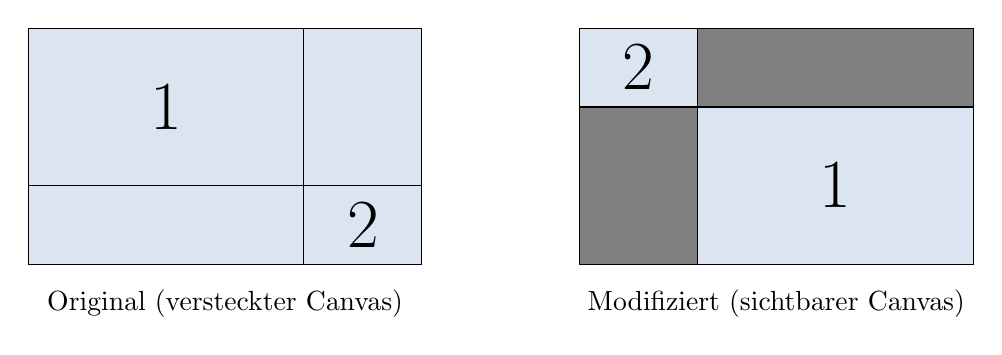
\begin{tikzpicture}

\definecolor{myblue}{RGB}{219,229,241}
\definecolor{mygray}{RGB}{128,128,128}

    %Farben
    \fill [myblue] (0,0) rectangle (5,3);

    %Rechteck mit Kreuz
    \draw (0,0) -- ++(5,0) -- ++(0,3) -- ++(-5,0) -- cycle;
    \draw (3.5,0) -- ++(0,3);
    \draw (0,1) -- ++(5,0);
    
    %Labels
    \node at (1.75,2) {\Huge 1};
    \node at (4.25,0.5) {\Huge 2};
    \node at (2.5,-.5) {Original (versteckter Canvas)};
    
%Rechte Seite
\begin{scope}[xshift=7cm]

    %Farben
    \fill [myblue] (0,0) rectangle (5,3);
    \fill [mygray] (1.5,2) rectangle (5,3);
    \fill [mygray] (0,0) rectangle (1.5,2);
    
    %Rechteck mit Kreuz
    \draw (0,0) -- ++(5,0) -- ++(0,3) -- ++(-5,0) -- cycle;
    \draw (1.5,0) -- ++(0,3);
    \draw (0,2) -- ++(5,0);
    
    %Labels
    \node at (0.75,2.5) {\Huge 2};
    \node at (3.25,1) {\Huge 1};
    \node at (2.5,-.5) {Modifiziert (sichtbarer Canvas)};
    
\end{scope}
\end{tikzpicture}
\end{figure} 